\documentclass[]{article}
\usepackage{listings}
\usepackage{graphicx}
\setlength\parindent{0pt}
\setlength{\parskip}{1em}
%opening
\title{Visualizing High-dimensional Ball-Embeddings
	while Keeping Topological Relations}
\author{Jan Scheffczyk \\ Oliver Leuschner \\ Joanna Polewczyk}
%

\begin{document}

\maketitle

%150-250 words
\begin{abstract}
	Region-based embeddings have been proven to be useful in knowledge graph reasoning. Existing visualization tool cannot preserve topological relations among high dimensional regions. We present a tool for visualizing high-dimensional balls that keeps topological relations after their dimensions are reduced to 2-dimensions. The first version of this tool provides four functions as follows: (1) Simple diagrammatic reasoning for syllogism; (2) diagrammatic reasoning with back-ground knowledge; (3) visualizing the construction process of ball-embeddings; (4) providing a web-service to impose a taxonomy structure onto its vector embeddings with zero-energy loss. A demonstration video of this tool is available at \dots. 
	
\end{abstract}
%
%
%
\newpage
\section{Introduction}

Bing able to learn from data, and robust to noisy inputs, Deep-Learning has been successful in a variety of AI tasks that have frustrated classic symbolic approaches for decades, such as object classification, machine translation, voice recognition, question-answering \cite{LeCunNature15}. However, Deep-Learning  Systems lack of explainability, can be fooled \cite{BiDAF16,JiaLiangaL17,Belinkov17}, and normally need much more learning data than human does \cite{tenenbaum15}. This introduces potential dangers into safety critical applications, such as autonomous driving. Introducing innate structures into Deep-Learning system has been advocated, and listed as one of the AI research topics in the Townhall meeting at AAAI-19, so that Deep-Learning research shall solve logical reasoning tasks (System 2 of mind) \cite{Kahneman11,benjio19}. As logical reasoning, such as Syllogism, is better represented by inclusion relations among regions, instead of translation among vectors \cite{Venn1880,diagram95}, recent researches have been attempting to promote vectors into regions to improve performances of logical query, triple classification, link prediction of Knowledge Graph \cite{dong19iclr,dong19,li2019smoothing,JuanziEmnlp18,ren2020}.   

% Though a powerful tool for learning from data, Deep Learning limits itself in representing everything as vectors, and can only approximate symbolic representation and reasoning. This limitation can be approached by promoting vector embeddings to ball embeddings. Vector embeddings of nodes in a taxonomy structure can be promoted into balls in higher-dimensional space, such that (1) each vector embedding is well preserved by the central point of a ball; (2) child-parent relations are precisely encoded by inclusion relations among balls. Significant results are obtained in experiments on unifying word-embeddings with hypernym trees and on unifying entity-embeddings learned from knowledge-graphs and tree structures. Being able to precisely imposing external symbolic structures onto Deep Learning systems not only paves the way towards resolving the antagonism between connectionism and symbolicism in the literature, but also has tremendous value in real applications. For example, being able to impose traffic rules onto autonomous driving cars would ultimately solve the safety issue.  

% Taxonomy, as a classification of concepts, exists in almost every disciplinary, such as file systems in computer science , government organization of a country, classification of viruses, plants, and animals. 

% Ball embeddings are rigorously constructed by a sequence of geometric transformations under the  condition that the loss function of the embedding must be zero, which is a condition that is not required and has not been targeted by Deep Learning approaches. This also raises the visualization problem of ball embeddings. 
The popular  tool t-NSE \cite{Maaten08} for visualizing vector embeddings cannot be directly applied for visualizing ball embeddings, for the dimensional reduction process of t-NSE does not guarantee the topological relations among balls. In this paper, we demonstrate an open source system that is able to visualize ball embeddings while keeping their topological relations. The main contributions of this system are as follows: (1) it has an vivid interactive user interface that can be used for diagrammatic reasoning among taxonomy; (2) it provides an effective and friendly approach for debugging the geometric construction process of ball embeddings; (3) it provides a batch service that accepts a large scale input for construct ball embeddings. 

\section{N-Balls embeddings}
\label{sec::ball}
Hierarchies or in other words trees can be expressed by ball embeddings. The largest N dimensional sphere corresponds to the root node of the tree. The direct children of the root node are represented by smaller spheres that are contained within the sphere of the root node. Hierarchies are an important part of natural language and signifies a type of relationship with another word. For example sparrow duck or Eagle are all of the type bird. In linguistics this is called a hypernym and hyponym relationship where the type of, in our example the bird, would be the hypernym and the concrete realizations of that type, in our example sparrow or a duck, would be some hyponyms of bird. It is self evident that having this kind of hierarchical information can be useful when creating a rule-based natural language processing tool. Unlike stochastical or learning based methods hierarchical structures do not come with an error rate or in other words we can always determine if a note is a child (hyponym) of a word that we are interested in or not. For example if we were to write a tool that needs to identifies cities within a certain region then the results most certainly have to be direct or indirect hypnonym of the word city.
\par
While rule-based natural language processing have been studied and applied for many decades now recently machine learning specifically deep neural networks have produced stunning results that seemed almost impossible with the traditional rule-based methods. However to actually use words or sentences in a neural network we first have to convert the input into to a vector that we can train our model on. This was first explored in the word2vec paper. The goal is to create a dense vector representation for each word. They start off by creating a sparse representation also known as one hot encoded. For this they determine all words used in their text corpus and create a vocabulary from that. Then every word can be represented by a vector of the length of the vocabulary that only contains a single entry 1 and all of her entries are 0. This allows us though in a very inefficient way to feed any word or even a sentence, a concatenation of these vectors, into a neural network. Further they assume that similar words have a similar context. For example in "Can you *blank* me the train station." we can fill this gap with lead, guide,show and all of them express a similar meaning. We can then train a neural network to represent every word with a limited dimension of our choosing. Common vector dimenions are 50, 100,300,500. This works remarkably well and allows us to explore relationships beyond simple hierarchies. In the original paper for example they could use the word vectors of Paris-France+ Italy=Rome. This approach has been extended multiple times for example glove. As with all learning based methods there is no guarantee that certain relationships that we observe in our language are actually projected into the word vector space. 

N-Ball and beddings combines both approaches to the reliability of a hierarchical based system in combination with the power and flexibility that is encoded into the word vectors. This is achieved by extending the word vectors and conceptually adding a sphere to the end of each of them. In the next step we need to ensure that the word embedding actually adhered to the hierarchical structure that we want to embed into them but at the same time we wish to preserve the vector of it has been assigned by the word embedding of our choice. This is done by adding more dimensions to these word vectors by only using homothetic transformations.

\section{The Architecture}
\label{sec::arch}
Here we will describe the basic information flow between the user interface given on the website, the Web server and the processing of the request. In order to display any kind website we first need to set up a Web server that serves HTML files along with their corresponding CSS and JavaScript files. As discussed previously we chose to use flask for this task as it allows us to stay in the Python ecosystem. We created a basic HTML website that provides a input field as well as some basic information about the project says that the user can understand the idea of the project and then proceed to either execute the given example or come up with his own. 
The user provides a tree structure which you would like to embed into a word embedding. Using statements with a fixed structure
E1 is E2
E1 is NOT E2
provides a simple way to describe a single hypernym, hypnoym relationship in a form that is both human readable and can be easily passed internally. Instead of using the input field the user can also upload a text file where each line contains a single hyper new statement. While this does provide a good way to intuitively define small tree structures we have to make a few assumptions in order to do the actual visualization. Both the underlying word vectors as well as the algorithm to create the N ball embedding is now assumed by our system to be the ones used in the original paper [CITE]. Alternatively the user can upload a Json file where he not only provides the tree structure but can also provide his own N ball embedding's along with the construction steps. With this we can create the visualizations for any Ball embedding. For the use of a simple json format should allow any application to quickly output the required attributes. 
At this point we have the user input which contains a list of entities as well as their relationship with each other henceforth abbreviated simply with input. The more specific case that also includes N-ball embedding will be handled basically the same with the difference that we can skip the steps required to compute that embedding ourselves. As described in section \ref{sec::redis} instead of handling the request directly we will create a task and place it into a task to to allow for direct feedback.  

Once the server is ready to perform the task, or in words once all of her tasks have been completed, we are ready to prepare the input sets that can be given to the existing N-Ball embedding framework. The existing framework provides a CLI interface and in order to keep changes to that framework to a minimum we opted to write a small API that simply translates CLI back to a Python interface. We further make sure that the required word embedding's are present and if not simply download them for convenience. The original framework creates a number of files for each embedding it computes. To ensure that tasks do not collide with each other as well as to ensure that results will be available after a task has been completed we ensure that every task gets a separate folder. Currently these folders are kept indefinitely and are named by random integer, also see EXTENSION. Finally we can ask the framework to generate the embedding.

Before we can do any kind of visualization we first need to reduce the dimension of the now extended word embedding down to 2D. For this we use the PCA reduction method explored and implemented by a previous project. Besides simply computing the 2D PCA embedding the project further try to resolve all instances which now violate the hierarchical embedding due to the PCA prediction. Finally this leaves us with both the high dimensional N ball embedding's as well as their fixed 2D projections.

We cannot take these 2D projections and generate drafts for them says that the user can interactively explore the results of the N ball embedding's. To allow for interactivity this has to be done with JavaScript. Fortunately the Python library plotly also has a JavaScript implementation. This allows us to generate all necessary shapes and markers within the Python code and and then later render them on the website. For more detail see section \ref{sec::plotly}.

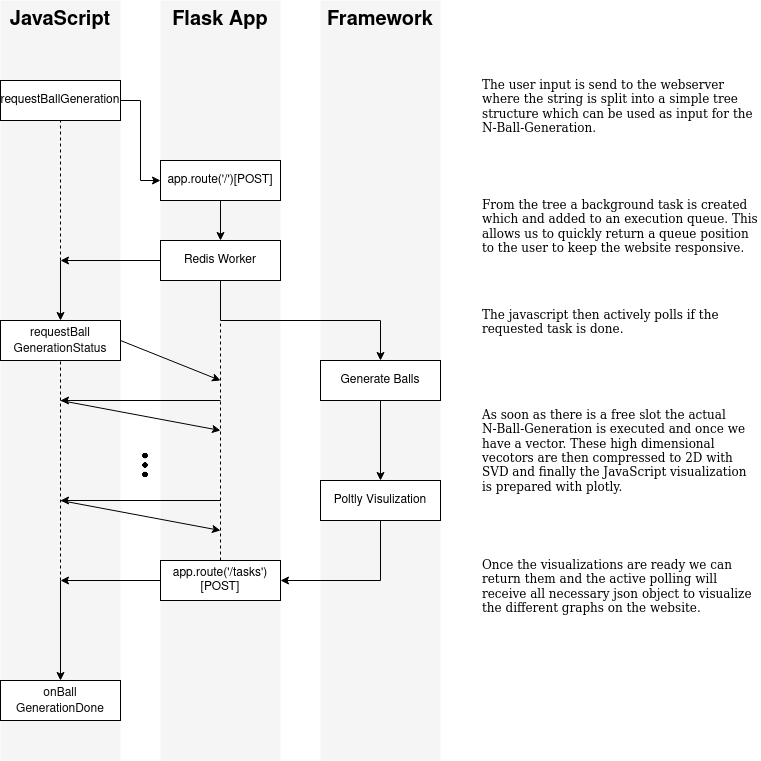
\includegraphics[width=\textwidth]{res/overview.png}
To get these results back to the user without the need to reload or redirect website we are using asynchronous AJAX requests. As soon the user submits either his input form or a file we send a AJAX request to the Web server which is immediately returned along with information of the task ID that the user has been assigned as well as which task you this tasks resides in. With these two inflammations the web client can then periodically request to get a status update on his tasks progress. This update request is answered with his current queue position or once a task is completed with the results of our plotly visualization. The realization results are passed back as a Jason file which will be passed in the JavaScript and passed into a JavaScript plotly instance allowing us to display the different graphs.

\subsection{Flask}
\label{sec::flask}
In order to provide a easily accessible demonstration website or visualization and interactive debugging tool is available through a website. As the original N-Ball embedding is implemented in Python, flask was chosen as a web framework.  Flask is a Python based micro framework and as such does not require any additional libraries and is readily available through the python package manager. 
As is convention with a flask application we provide HTML templates in the template folder. These templates are just the basic HTML skeleton which defines where and in which order a different graphs, input fields and text fields will be inserted on the website. The basic formatting is done through the CSS bootstrap framework. We further extend on this with our own CSS file which can be found under templates/static/css along with the JavaScript code under templates/static/js. 


\subsection{Redis}
\label{sec::redis}
For every input the system needs to generate the corresponding ball embeddings, save each step in the construction process, reduce the dimension of the embedding down to two dimensions for visualization and where possible resolve overlapping that results from the dimensionality reduction. Depending on the size of the input tree this process can take anywhere from a few seconds to a few minutes. With a naïve implementation the Web server would simply do all of these tasks before sending back the response to the user. This would not only leave she was awaiting with no feedback but even more importantly the server would not be reachable at all during that timeframe for other users. While works well for single user it is obviously unacceptable for a publicly available website. We need to make sure that a large will not block the Web server for everybody else for minutes possibly even hours. Therefore we need to decouple the serving of the website from the actual computation of the ball embeddings. This is done by using a task queue.
We chose to use a commonly used task queue named redis. This allows us to create a task queue so when the user requests the computation of a ball embedding we added to the task you and immediately returned to the user to tell him that we received his request and that he has been placed into the task queue. Once the task is complete the results can be sent to the users browser through AJAX without the need to refresh or redirect the website. This allows for seamless display of the results. While the website will return immediately and give the user adequate feedback this still allows a single user to effectively block the queue. As he places a large request once the Web server starts computing this task it will not work on tasks that have been requested later. In order to keep the websites response time for small requests low we introduced a second high priority queue that is reserved for small to moderate input sizes to ensure that users they want to experiment with the service will not be blocked by a single large request.
\begin{lstlisting}
r = redis.Redis()
q_high = Queue("high", connection=r)
q_low  = Queue("low", connection=r)  
\end{lstlisting}

\section{Services}

\subsection{words meaning and etimology}

\subsection{Simple Diagrammatic Reasoning}

Ball embeddings allow for strict reasoning and logical queries. This can be demonstrated with our tool. The user can input hypernym relationships in plain English such as "socrates is human, human is animal" we display that relationship as seen in figure X. Similarity system also handles exclusion such as "soccer is not human,human is mortal" as seen in figure X. Once these relations have been enforced on the sufficiently large corpus, ideally for all words present in the underlying word embedding, this allows for strict logic varies which are otherwise impossible in neural networks.

\subsection{Diagrammatic Reasoning with Background Knowledge} 
\begin{itemize}
	\item user input: Soccer is not human, human is animal
	\item  user query: what is the relation between Soccer and animal
	\item  system replaces `Soccer is not human' with `Soccer is entity', system adds 'animal is entity' by searching background knowledge
	\begin{verbatim}
	>>> from nltk.corpus import wordnet as wn
	>>> soccer = wn.synsets('soccer')
	>>> soccer
	[Synset('soccer.n.01')]
	>>> soccer = wn.synsets('soccer')[0]
	>>> soccer
	Synset('soccer.n.01')
	>>> human=wn.synsets('human')[0]
	>>> human
	Synset('homo.n.02') 
	>>> soccer.lowest_common_hypernyms(human)
	[Synset('entity.n.01')] 
	>> % check 'animal' and 'entity'
	>> ..
	\end{verbatim}
	\item  system draw: (1) Soccer ball outside animal ball, (2) human ball inside animal ball; (3) they are inside entity ball 
	\item system merges (1), (2), and (3)  
	\item system conclude: Soccer is not animal.
\end{itemize}

\subsection{Visual Debugging}
Enforcing a relational structure onto word embedding is a difficult task. Similar to a code-debugger we provide a visual feedback for every construction step which; (1) allows the viewer to retrace and understand the construction process and as such serves as a valuable teaching tool; (2) enables developers to optimize {and correct their ball embedding construction.
	
	Since we only consider hierarchical structures in this paper we can guarantee that any valid state can be visualized on to a two dimensional canvas. In order to achieve this we first construct a set of nonoverlapping circles that perfectly represents the hierarchy that is to be encoded into the ball embeddings. Then within each construction step we either display the previously computed perfect representation or enforce any overlapping's that have been recorded in the ball embedding construction history.
	
	\subsection{Batch Service}
	
	\begin{itemize}
		\item user provide her/his name and contact email.
		\item user input: a tree structure, vector embeddings of tree nodes
		\item System will construct ball embeddings at backend, and send the user the link fo the final ball embeddings  
	\end{itemize}
	
	\section{Conclusion and Outlooks}
	
	link to the video
	
	
	%
	% ---- Bibliography ----
	%
	% BibTeX users should specify bibliography style 'splncs04'.
	% References will then be sorted and formatted in the correct style.
	%
	% \bibliographystyle{splncs04}
	% \bibliography{mybibliography}
	
	\bibliographystyle{plain}
	\bibliography{XBib_NN,XBib} 

\end{document}
